\documentclass[conference]{IEEEtran}
\IEEEoverridecommandlockouts
% The preceding line is only needed to identify funding in the first footnote. If that is unneeded, please comment it out.
\usepackage{cite}
\usepackage{amsmath,amssymb,amsfonts}
\usepackage{algorithmic}
\usepackage{graphicx}
\usepackage{textcomp}
\usepackage{xcolor}
\usepackage{gensymb}
\usepackage{listings}
\usepackage[framed,numbered,autolinebreaks,useliterate]{mcode}
\def\BibTeX{{\rm B\kern-.05em{\sc i\kern-.025em b}\kern-.08em
    T\kern-.1667em\lower.7ex\hbox{E}\kern-.125emX}}
\begin{document}

\title{A Probabilistic Model for Demonstrating High Path Planning Success Rate in Autonomous Capsule Robots for Bronchoscopies}

\author{\IEEEauthorblockN{Arjan Gupta}
\IEEEauthorblockA{\textit{Robotics Engineering} \\
\textit{Worcester Polytechnic Institute}\\
Worcester, MA, USA \\
agupta11@wpi.edu}
}

\maketitle

\begin{abstract}
This manuscript describes a probabilistic view of analyzing the
possible paths that an autonomous robot may take when traversing
through bronchi. We will consider a section of
the lung, as a model that can be expanded upon using our work. Using
the technique of rapidly-exploring random trees (RRT),
we aim to lay down some benchmarks that can be used
by clinical experts to meet the goal of the bronchoscopies
they perform.
\end{abstract}


\begin{IEEEkeywords}
    capsule robot, autonomous bronchoscope, path planning, benchmark parameters
\end{IEEEkeywords}

\section{Introduction}
Bronchoscopies play a vital role in diagnosing a range of pulmonary
issues. For example, tumor detection is an important cause for an
endoscopy performed by a pulmonologist. However, low diagnostic
yields is an existing problem in transbronchial biopsies
\cite{Rivera2013},\cite{WangMemoli2012},\cite{Mehta2018},\cite{Ost2016}.
Among the many solutions to address this
problem, robotic-assisted bronchoscopy is a promising
and ever-growing method\cite{Lu2021}. In the variety of types of robotic
bronchoscopies, a capsule-robot has potential and can be expanded upon in
many ways. For example, the existence of the PillCam COLON capsule has
shown promise in the last decade\cite{Adler2011}. Although again in
the realm of colonoscopy screenings, a capsule endoscopy has shown
to be considerably more cost-effective as compared to traditional
methods\cite{Hassan2008}.\\

While rigid and fiberoptic 
methods remain the dominant methods of performing pulmonary
endoscopies\cite{Lu2021}, they also require highly skilled
operators in order to be safe\cite{Stahl2015}. However,
given the forecasted shortage in the physician workforce
of the United States\cite{Zhang2020}, it is imperative
to look for alternative solutions. Autonomous endoscopies
are one such solution. In fact, autonomous capsule robots
have already been trained using reinforcement learning
for usage in endoscopies\cite{Turan2019}.\\

However, at
the time of the scribing of this manuscript, the existing
literature does not show any preliminary benchmark information
about this type of robotic bronchoscopy. If clinical operators
hope to use autonomous capsule robots for bronchoscopies, there needs
to exist guidelines on tuning the autonomous robot such that a
high success rate for biopsy yield can be achieved.
\textit{
The primary objective of this study is to show a
simple probabilistic method
to achieve over 98\% success rate of an autonomous capsule
robot to find a given destination in the human bronchi.
We will use rapidly-exploring random trees to set up a model that
can establish parameters which can be tuned to achieve a high success
rate.}

\section{Materials and Methods}

\subsection{Set up for the model}
First we use a simple figure that delineates occupied and free zones
of a human pulmonary region. Such a figure is shown in Fig~\ref{given-lung-fig}.
The green region is the the area where the capsule robot is free to move, and
the black regions are the `occupied' zones, signifying the walls of the
organ.

\begin{figure}[h]
    \centering
    
\includegraphics[scale=0.11]{939-Oblique.png}
    \caption{A basic model of the human lung}
    \label{given-lung-fig}    
\end{figure}

The capsule robot's dimensions are roughly 10 mm long capsule with 5 mm in diameter,
but for the sake of model simplicity, the dimensions are ignored in the
path planning. We assume that the robot can start anywhere near the trachea
and have a goal position near the end of the narrow bronchi.

\subsection{Occupancy grid and start/goal positions}

Next, we read in the image using MATLAB's \textit{imread} function. Now
that we have a raw byte version of the image, we convert it to
a gray-scale image. By default MATLAB reads this in as the colored
portion marked as black, so our next step is to invert the image,
which we can do with a simple logical invert on the image matrix.
At this point, we can use MATLAB's \textit{binaryOccupancyMap} function
to create an occupancy grid, so that we can determine which
regions are occupied and free. The image was given a resolution
of $10^4$, in order to model a more realistic size of the lung.

Furthermore, the start position of the robot was randomized. In our
image, $750 \times 10^{-4}$ is roughly the y-height of the trachea.
However our robot could start anywhere along the x-width of this trachea,
therefore we use the \textit{randi} function to randomly select an
x-position anywhere between $685 \times 10^{-4}$ and $800 \times 10^{-4}$.

To select random locations for the goal, we first randomly selected
the left or right narrow airway. If the left one was selected, we
selected a y-height of $660 \times 10^{-4}$ and randomly generated
the x-position between $415 \times 10^{-4}$ and $445 \times 10^{-4}$.
If the right narrow airway was selected, we randomly generated the x-position
between $540 \times 10^{-4}$ and $560 \times 10^{-4}$.

\subsection{Dubins and Reeds-Shepp Curves}

Next, we model our state space for the path planning algorithm based
on Reeds-Shepp Curves. To understand it, we first describe the Dubins
path. A Dubins path analyzes a simple car model, and generates
the shortest path between two 2D poses $(x, y, \theta)$. The paths
can have three segments, right turn (R), left turn (L), straight line (S).
Based on optimization techniques, the possible path can have the the following combinations,
\[
    \{L_\alpha R_\beta L_\gamma, R_\alpha L_\beta R_\gamma, L_\alpha S_d L_\gamma, L\alpha S_d R_\gamma, R_\alpha S_d L_\gamma, R_\alpha S_d R_\gamma \}
\]

where $\alpha, \gamma \in [0, 2\pi), \beta \in (\pi, 2\pi)$, and $d \geq 0$. An example of
$R_\alpha S_d L_\gamma$ is shown in Fig~\ref{dubins-eg}.

\begin{figure}[h]
    \centering
    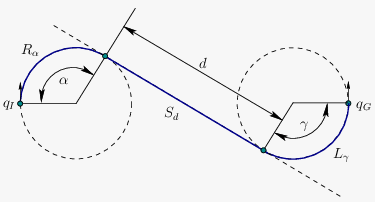
\includegraphics[scale=0.5]{dubins-img.png}
    \caption{An example of $R_\alpha S_d L_\gamma$ Dubin's curve}
    \label{dubins-eg}
\end{figure}

The Reeds-Shepp curve is the same as Dubins curve, except that reverse direction
movement is now allowed. Therefore, the sequences of motion primitives can be arrived
at by using the Dubins combinations, and applying permutations using $R^+, R^-, L^+, L^-$,
where the positive and negative signs denote forward and reverse motion.

In our MATLAB code, we specify that we want to use the \textit{stateSpaceReedsShepp} object with
the bounds given by the \textit{binaryOccupancyMap}. We specify a minimum turning radius
of $20 \times 10^{-4}$.

\subsection{Validation and path planning}

We additionally set up a \textit{validatorOccupancyMap} with a validation distance
of $5 \times 10^{-4}$. Finally, we are ready to call our rapidly-exploring random trees
planner, \textit{plannerRRT}. For the RRT algorithm, we set our maximum branch connection
distance to be 10 times our validation distance. We also set our maximum iterations at
$9 \times 10^3$.

After this, we plot the various branches of the RRT algorithm, as well as the path, if it is
found. We also show our starting and goal positions in the plot.

\section{Results}

An example plot of our RRT algorithm is shown in Fig~\ref{trial24-fig}.

\begin{figure}[h]
    \centering
    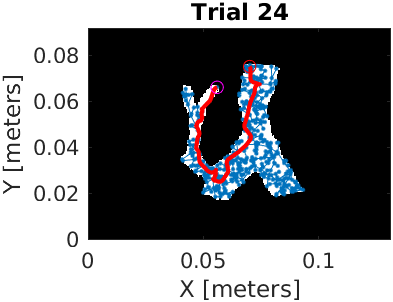
\includegraphics[scale=0.85]{trial24.png}
    \caption{An example trial of the RRT algorithm}
    \label{trial24-fig}
\end{figure}

The RRT algorithm we have written was run in batches of 24 trials, and plotted as subplots.
For each path successfully found path, we incremented the total successes by 1. After all
24 trials were run, we divided the number of successes by 24 in order to calculate the
success rate. An example of a perfect success rate is shown in Fig~\ref{trial-batch-img}.

\begin{figure}[h]
    \centering
    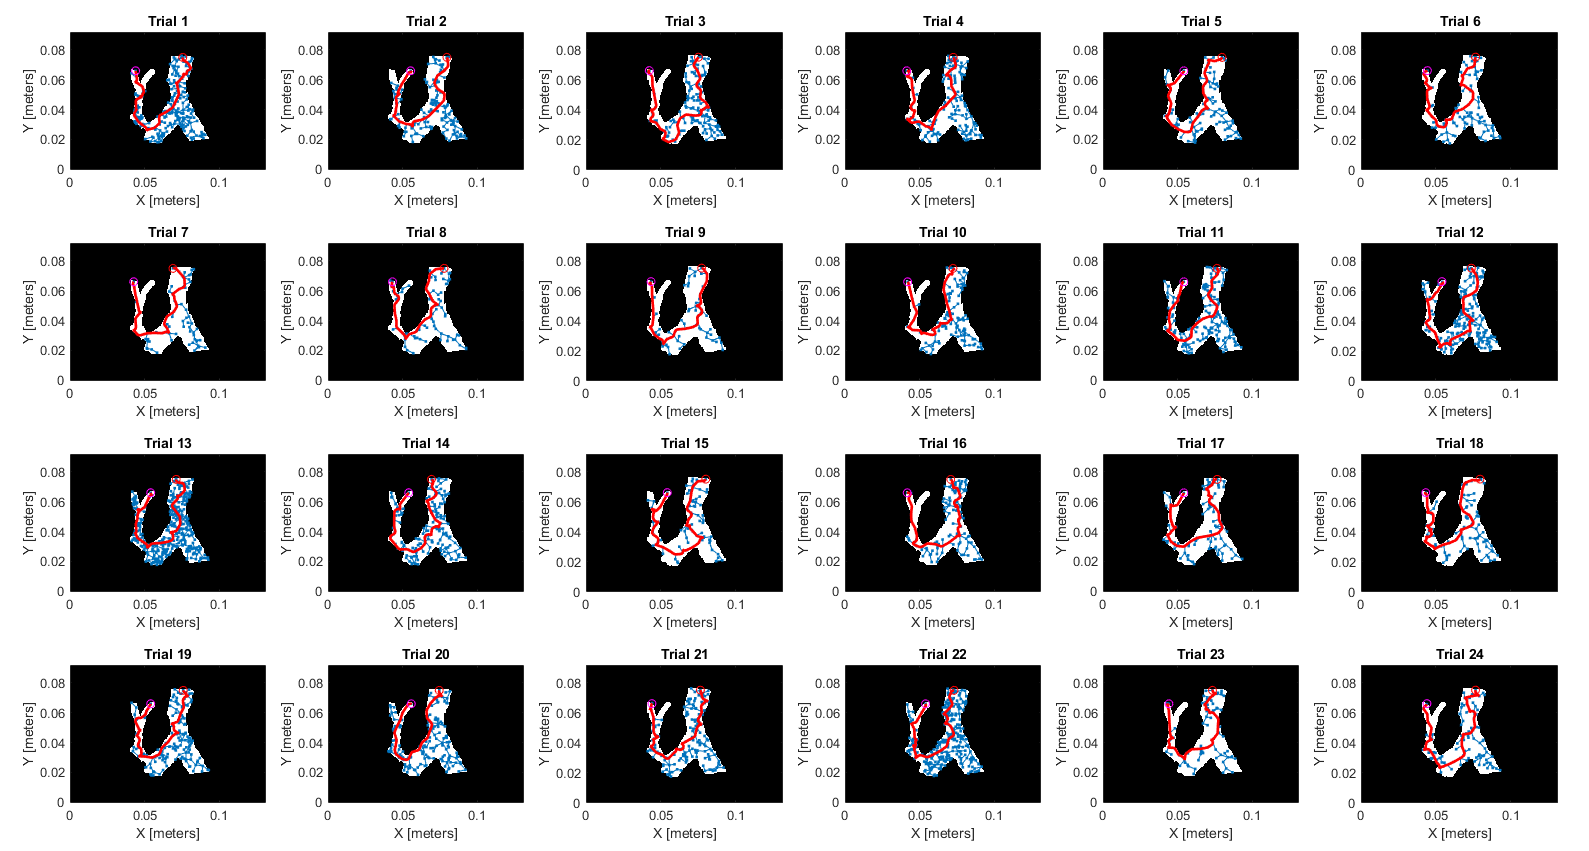
\includegraphics[scale=0.21]{random-trials.png}
    \caption{An example of a batch of trials with 100\% overall success rate}
    \label{trial-batch-img}.
\end{figure}

These batches of 24 trials were then run 5 times in order to average the success rate. In
our final results, we obtained 2 results of $95.83\%$ success rate, and 3 perfect success
rate batches. We have formulated Table~\ref{rrt-batch-table} in order to summarize the results.
From this table, we can average our overall success rate as $98.33\%$.

\begin{table}[h!]
    \begin{center}
        % \resizebox{0.8\columnwidth}{!}{%
        \begin{tabular}{||c|c|c|c|c||}
        \hline
        Trial Batch & Success Rate \\
        \hline\hline
        1 & $100.00\%$ \\
        2 & $95.83\%$  \\
        3 & $100.00\%$ \\
        4 & $95.83\%$ \\
        5 & $100.00\%$ \\
        \hline
        \end{tabular}
        % }
    \end{center}
    \caption{Batch results for RRT algorithm}
    \label{rrt-batch-table}
\end{table}

\section{Discussion}
In the opinion of the author, this homework problem set was insightful. The given methods
can be applied to analyze the reward system for reinforcement learning agents in autonomous
capsule robot navigation.

\section{Appendix}

\subsection{Success rate assessment script}

\lstinputlisting{assess_capsule.m}

\subsection{Path planning for capsule robot}

\lstinputlisting{capsule.m}

\subsection{Callback function for goal proximity check}

\lstinputlisting{checkIfReachedGoal.m}

\bibliography{refs.bib}
\bibliographystyle{IEEEtran}

\end{document}